%!TEX root = ../thesis.tex
%*******************************************************************************
%****************************** Second Chapter *********************************
%*******************************************************************************

\chapter{Previous Work}
\label{ch:2}

\graphicspath{{Chapter2/Figs/Vector/}{Chapter2/Figs/Raster/}}

% **************************** Nomenclature **********************************
\nomenclature[c-1-x]{$x$}{Data points where $x=\{x_0, x_1, ..., x_{N-1}\}$}
\nomenclature[c-1-y]{$y$}{Labels for the dataset where $y=\{y_0, y_1, ..., y_{N-1}\}$}
\nomenclature[c-1-N]{$N$}{Number of features/dimensions of $x$}

\nomenclature[c-1-s]{$s_g$}{Sample standard deviation of the predictions}


\nomenclature[c-2-IC50]{$\mathrm{IC_{50}}$}{Half maximal inhibitory molar concentration}
\nomenclature[c-2-XC50]{$\mathrm{XC_{50}}$}{Half maximal effective or inhibitory molar concentration}
\nomenclature[c-2-EC50]{$\mathrm{EC_{50}}$}{Half maximal effective molar concentration}
\nomenclature[c-2-AC50]{$\mathrm{AC_{50}}$}{Half maximal effective molar concentration}
\nomenclature[c-2-Ki]{$\mathrm{Ki}$}{Half maximal molar concentration for half receptor occupancy}
\nomenclature[c-2-LD50]{$\mathrm{LD_{50}}$}{Median lethal dose}


%*****************************************************************************

In order to assit the understanding of the methodologies used by others within the field of active learning, a toy dataset has been created. It is based upon~\ref{eq:phantom} and has been shown in Figure~\ref{eq:phantom}. The $y$ values used within the algorithms have been combined with errors, $\epsilon{}\sim{}\mathcal{N}(0, 0.01)$.

\begin{equation}
  y = \sin{(x_0)}^{10} + \cos{(10 + x_0 x_1)}\cos{(x_0)}
  \label{eq:phantom}
\end{equation}

\begin{figure}[h]
  \begin{center}
    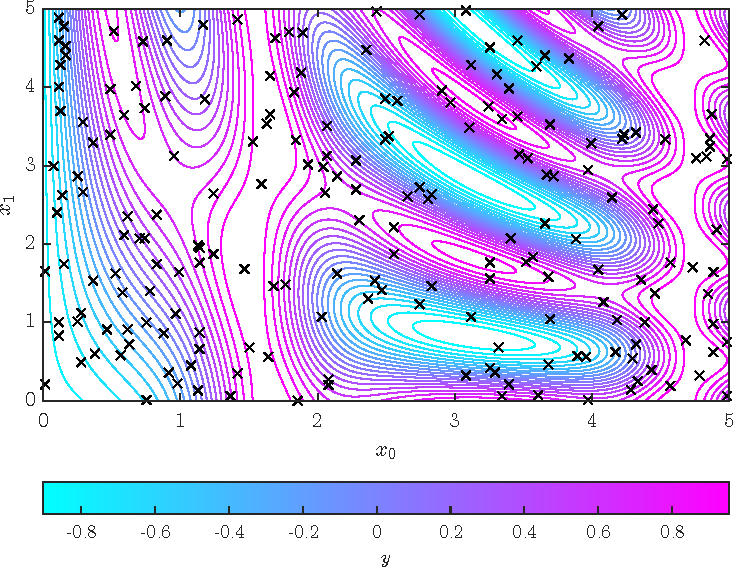
\includegraphics{phantomOverview.pdf}
    \caption[Example Dataset for Representation of Ideas]{Contour plot of the function used to demonstrate the algorithms presented in previous work. The crosses have been used to show the location of the 200 test data points used within this example.}
    \label{fig:phantom}
  \end{center}
\end{figure}

In order to assess the algorithms, the mean squared error (mse) has been used. Comparisons are made to the naive approach of random sampling, i.e. Monte Carlo sampling. Each algorithm will be given five random starting points, and attempted improvement will follow.

\section{Active Learning}
\label{ch:Active Learning}

There are several schools of thought regarding active learning. These can be separated into two distinct categories: current data and future predictions. The former of these is computationally cheaper, more complex t implement, and less adaptable to model changes, as will be apparent on description.

\subsection{Current Data}
\subsubsection{Uncertainty Sampling and Regions of Disagreements}
\label{sec:UncertaintySampling}

The simplest is applicable to cases in which a certainty is provided with each prediction. \textcite{Set09} suggests selecting the data point with the largest uncertainty according to the current model. This has been shown with the toy dataset, as demonstrated in Figure~\ref{fig:rodPhantom}.


\begin{figure}
  \begin{center}
    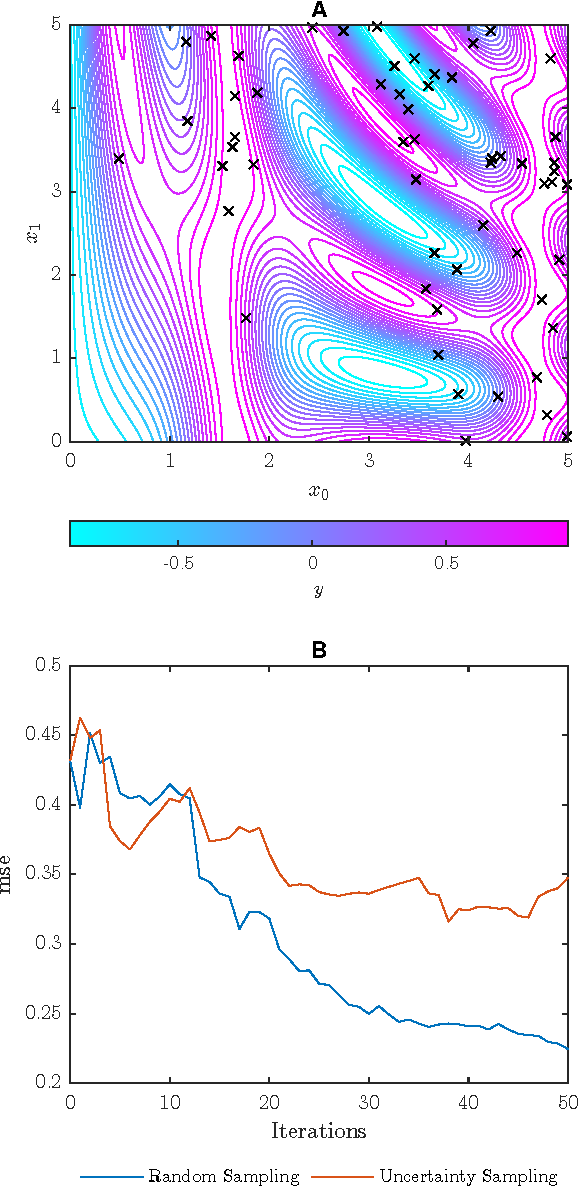
\includegraphics{rodPhantom.pdf}
    \caption[Uncertainty Sampling Demonstration]{The outcome of the investigating the areas of the highest uncertainty. An initial set of 5 random points was provided, and 50 further iterations were then carried out of sample size 1. A) Demonstrates the final set of points tested by the algorithm and B) shows the change in the mean squared error for the algorithm after each iteration.}
    \label{fig:rodPhantom}
  \end{center}
\end{figure}

Interestingly, Figure \ref{fig:rodPhantom}B shows how the mean squared error for the random sampling method performed to worse within the iterations tested. This is likely due to a bias in the use of linear models in fitting leading to large uncertainties surrounding areas with high curvature. Evidence to this is provided in Figure~\ref{fig:rodPhantom}A with a large proportion of the sampled points at areas of high curvature.

As addressed by \textcite{Set09}, this can be extended to any probabilistic model through \ref{eq:x_next1}. \textcite{Set09} also notes the use of information theory for probabilistic models(\ref{eq:info_uncertainty}), where $y_i$ refers to all possible categorisations for $x$. This derives from the principle that the greatest entropy requires the most information to encode, and thus the least certain. However, \textcite{Set09} fails to address non-probabilistic models in this instance, instead converting such models into probabilistic ones.

\begin{equation}
  \label{eq:x_next1}
  x_\mathrm{next}=\argmax_X{\left[s_{g(X)}\right]}
\end{equation}

In order to adapt non-probabilistic models into probabilistic ones, composite models may be used. These are an amalgamation of other models where the standard deviation of the individual models can be taken as the degree of certainty for a given point. This is commonly refered to minimising the region of disagreement, refering the spaces of discord within the hypothesis space. By minimising the region of disagreement between various models, a more coherent hypothsis space is sought leading to a more accurate model. Indeed, this was the method used in Figure \ref{fig:rodPhantom}. Mathematically, a set of $n$ models ${M = \{m_0,\ldots{}, m_{n-1}\}}$, with each model offering a precition of $\hat{m_i}$, ${\hat{M}=\frac{1}{n}\sum{\hat{m_i}}}$, and the sample standard deviation of $\hat{m}$ giving the uncertainty.


\textcite{Set09} suggests  third way of interpreting uncertinty. By taking the approach from information theory, \ref{eq:infoUncert} is settled upon. This directly states gives the point of highest entropy, suggesting by knowing the point provides the largest information gain. Notably however, this is difficult to implement with most models, as a probability distribution is required. This could be made simpler by approximating to a normal distribution.

\begin{equation}
  \label{eq:infoUncert}
  x_\mathrm{next}=\argmax_x{\left[\phi_A(x)\times{\left(\frac{1}{U}\sum{\simm{(x, x_i)}}\right)}^\beta\right]}
\end{equation}


% \subsubsection{Broad Knowledge Base}
% A second form stems from information theory. Here, the aim is to produce an evenly dispersed $x$ allowing a well-informed knowledge base. This prevents poor model choice from influencing the algorithm as was seen in \ref{fig:rodPhantom}. There are two paths to proceed: density and nearest neighbours.


% The former of these requires a definition of density in a sparsely populated space. As an analogy, although the density of a gas appears well-defined, it becomes non-smooth once the volume defined over is comparable to the distance between particles. Thus, a new definition is required.

% Alternatively, nearest neighbour requires little explanation. $x_\mathrm{next}$ is the unlabelled data point furthest from any labelled data point. The results of \ref{eq:inverseSim} can be seen in Figure~\ref{fig:b}.

% \begin{equation}
%   \label{eq:inverseSim}
%   x_\mathrm{next}=\argmax_x{\left(\sum{\frac{1}{\simm{(x, x_i)}}}\right)}
% \end{equation}

% \begin{figure}[h]
%   \begin{center}
%     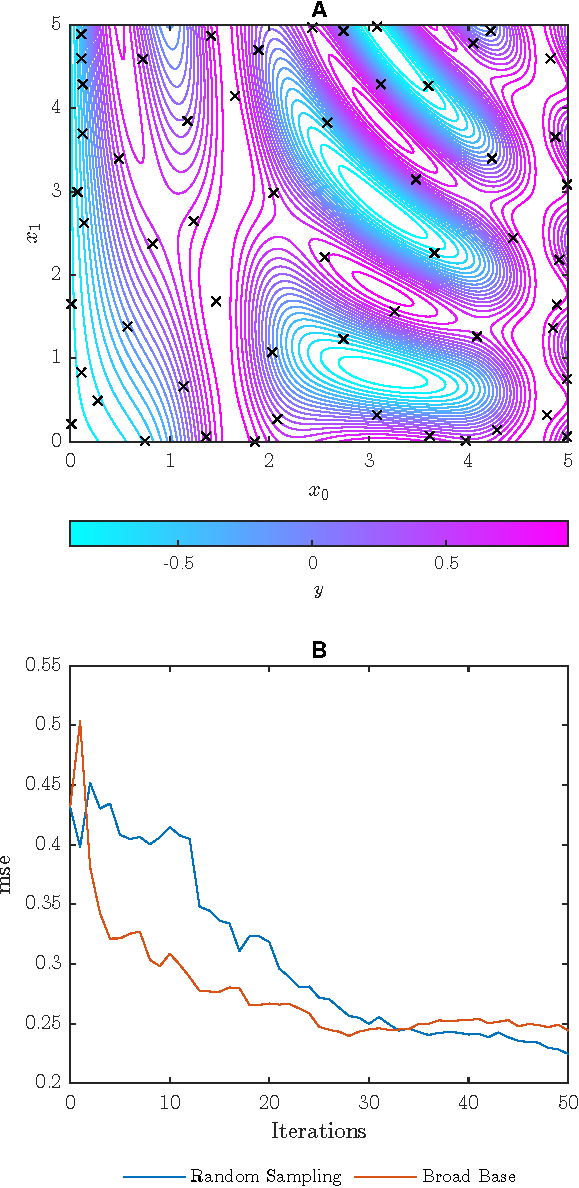
\includegraphics{broadPhantom.pdf}
%     \caption[Broad-Base Sampling Illustration]{The outcome of the investigating the areas of using a broad base. An initial set of 5 random points was provided, and 50 further iterations were then carried out of sample size 1. A) Demonstrates the final set of points tested by the algorithm and B) shows the change in the mean squared error for the algorithm after each iteration.}
%     \label{fig:b}
%   \end{center}
% \end{figure}


\subsubsection{Density Hotspots}
\label{sec:litRevDH}
Conversely, a density weighted model has been suggested, as it escapes the introduction of error from outliers (i.e.\ data points far away from alternative data points). \textcite{Set08} suggest (\ref{eq:Settles_density}) which can be broken down into two parts: a function for selection, $\phi_A$, and a function for similarity, $\simm$. The former arises from  another method described in this section. The latter requires a function to describe the similarity between data points.

\begin{equation}
  \label{eq:Settles_density}
  x_\mathrm{next}=\argmax_x{\left[\phi_A(x)\times{\left(\frac{1}{U}\sum{\simm{(x, x_i)}}\right)}^\beta\right]}
\end{equation}

\textcite{Set08} admit that $\simm$ is open for interpretation. It must also be recognised that this lays the foundation of a clusterisation algorithm. There exist many forms of these algorithms, with the results of several of these algorithms on toy data sets presented in Figure~\ref{fig:ClusterResults} \cite{SciClus}.

\begin{figure}[H]
  \begin{center}
    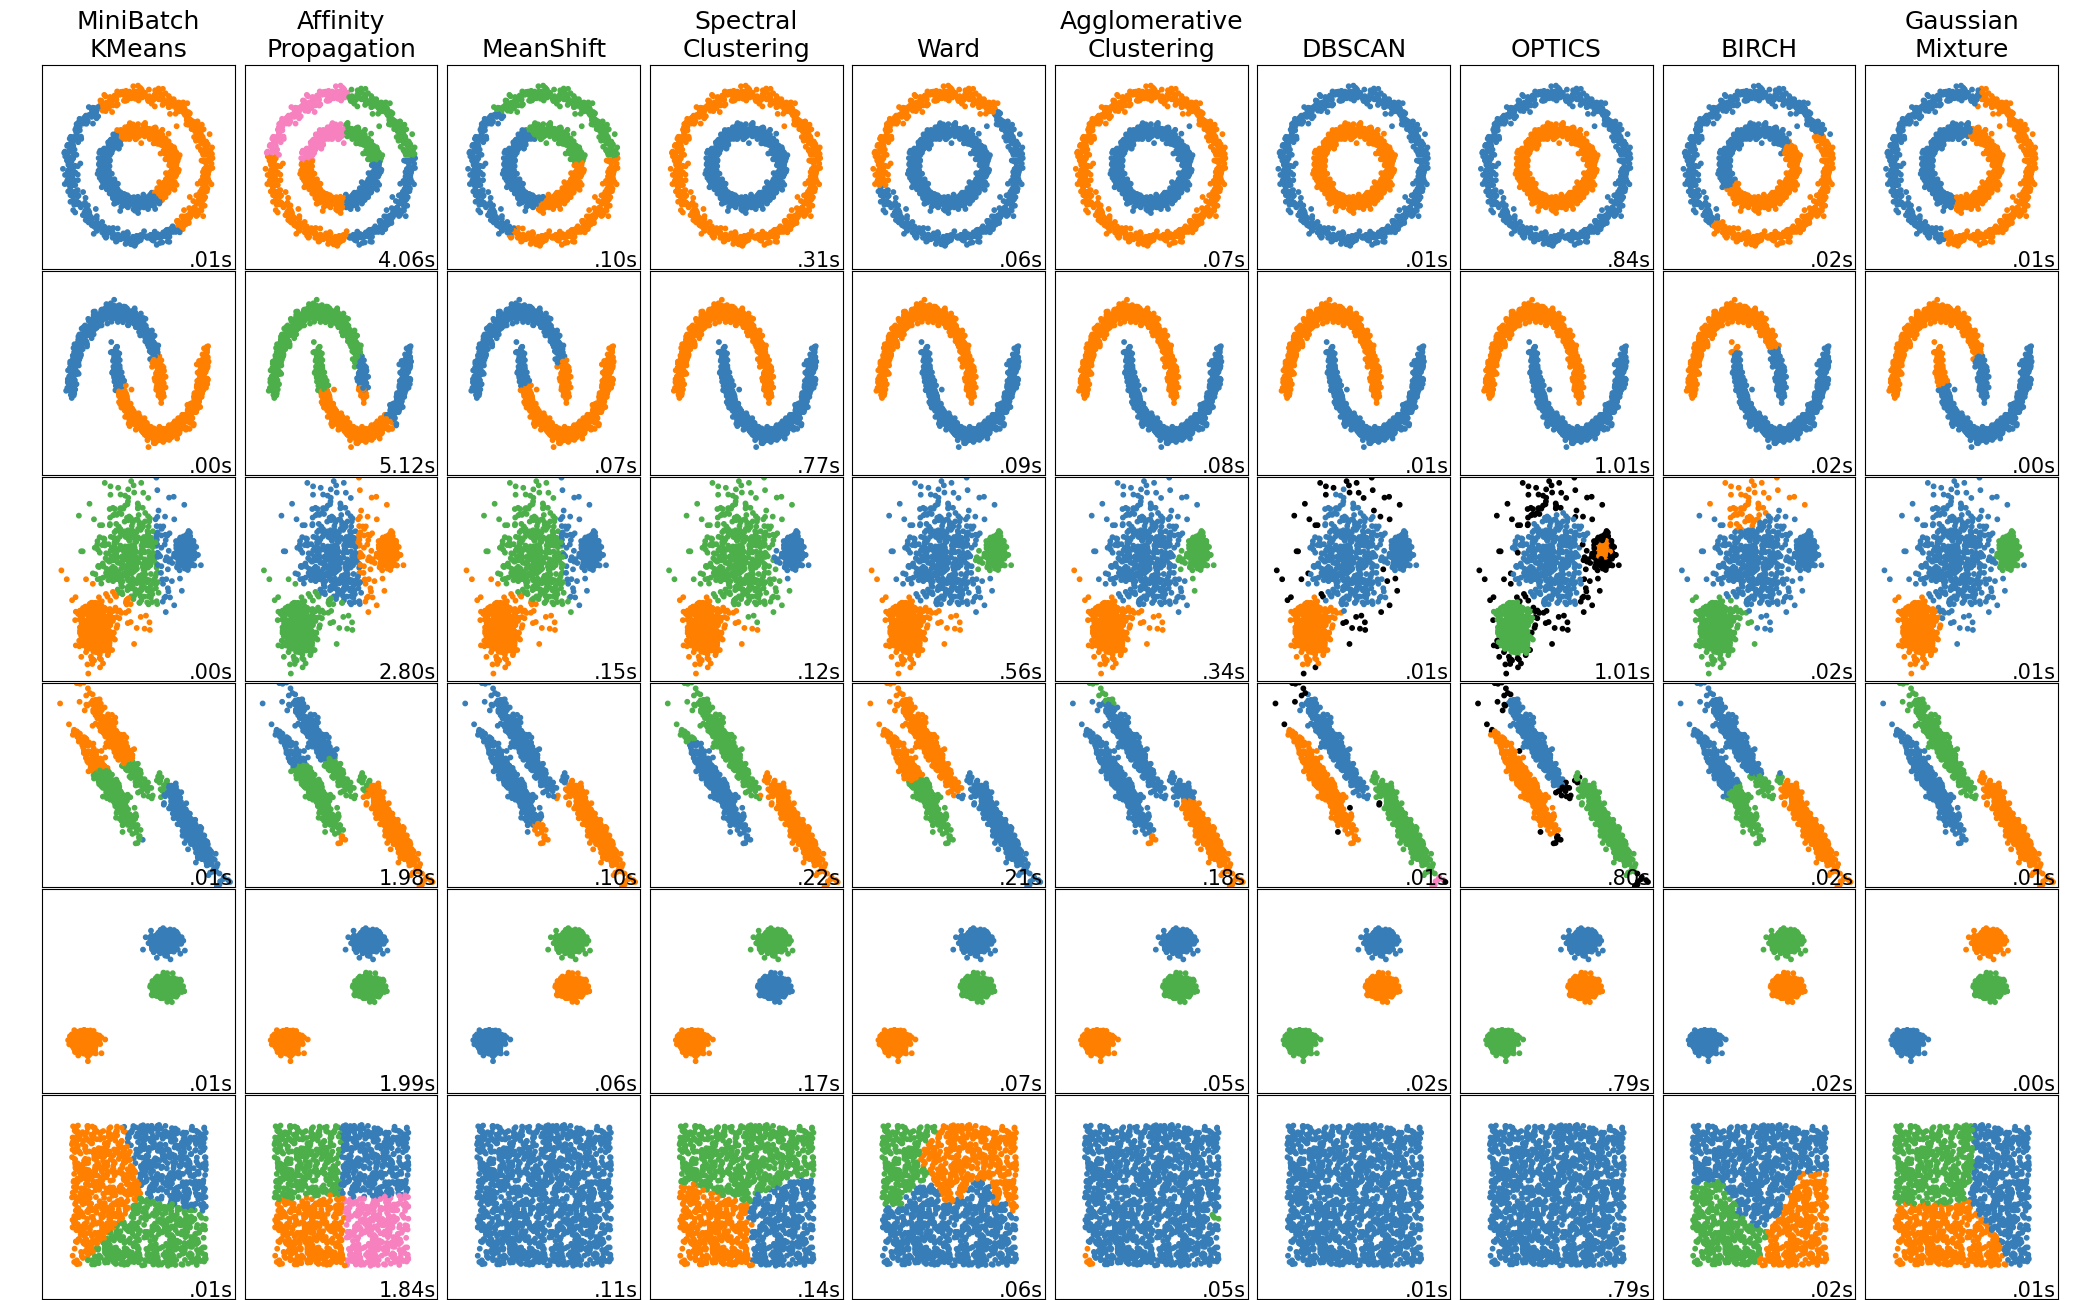
\includegraphics[width=\textwidth]{clusters.png}
    \caption[]{Clusterisation algorithms used on sample two-dimensional data sets to demonstrate resultant clusters.}
    \label{fig:ClusterResults}
  \end{center}
\end{figure}

As Figure~\ref{fig:ClusterResults} demonstrates, there are multiple different interpretations of the solution to the problem of clustering. The makers of the Sci-kit learn package also discuss the scalability of each algorithm \cite{SciClus}. In order to prepare a high number of features (beyond the two used within this section for demonstration) and large number of data points, it is required that the algorithm scales accordingly. Further, for an adaptive process, it is more suitable for an algorithm to be adaptive to differing distribution. This limits the suitable algorithms to K-Means, Ward and Birch - columns one, five, and nine of Figure~\ref{fig:ClusterResults} respectively. Results for Birch can be seen in Figure~\ref{fig:clusterPhantom}. This appears do well, although it must be noted that this is likely due to the similarity between Monte Carlo (random) sampling, and clusterisation. I.e. areas distant from previously gathered points face a high chance of sampling.

\begin{figure}[H]
  \begin{center}
    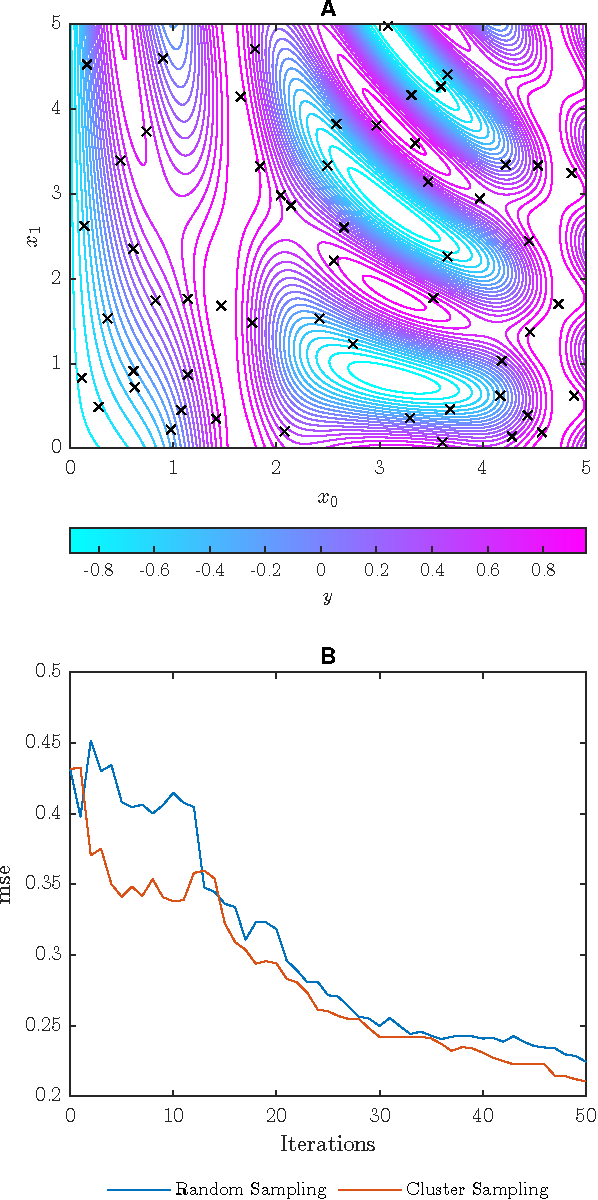
\includegraphics{clusterPhantom.pdf}
    \caption[Cluster Hotspot Sampling Illustration]{The outcome of the investigating the areas of using a cluster hotspot sampling methodology. An initial set of 5 random points was provided, and 50 further iterations were then carried out of sample size 1. A) Demonstrates the final set of points tested by the algorithm and B) shows the change in the mean squared error for the algorithm after each iteration.}
    \label{fig:clusterPhantom}
  \end{center}
\end{figure}

\subsection{Estimated Future}
These methods attempt to minimise a future attribute of the model. This works by predicting changes given with the inclusion of more data with a higher degree f theoretical underpinning that the sampling methods discussed thus far.

\subsubsection{Expected Model Change}
As the name implies, this method chooses points which are likely to have the largest impact on the final model. By instigating each potential point, the impact on the eventual model can be found. However, this requires a method for quantifying the model change.

\textcite{Set08,Set09} investigate models which can be trained "online": i.e. models which can use the previous iteration to reduce the time taken for convergence. They present a method called "Expected Gradient Length" (EGL) which has a couple of prerequisites: \textbf{1)} A probabilistic model is used \textbf{2)} Linear gradient based optimisation is used \textbf{3)} The model can be improved from previous iterations. Given these prerequisites, the problem becomes less computationally inexpensive given a small dataset or extensive parallelisation, and scales as $\mathcal{O}(n)$. However, it does have the distinct drawback of requiring close control of the data models used. Here, the length of the training gradient (the gradient used in re-fitting the parameters with gradient based optimisation) can be used as a measure of model change. In the case of a small model change, as is expected, the lenth of the training gradient can be written as ${\left\|\nabla{}l(\langle{}x, y_i\rangle{};\theta{})\right\|}$. Combining this with the probability distribution of $y$, the next sample to undergo labelling is given by \ref{eq:EGL}.

\begin{equation}
  \label{eq:EGL}
  x_{EGL}^*=\argmax_x{\sum_i{P(y_i|x;\theta{})\left\|\nabla{}l(\langle{}x, y_i\rangle{};\theta{})\right\|}}
\end{equation}


\section{Batch Active Learning}
Little literature exists with respect to batch active learning. Naive implimentation exist whereby the methods explored earlier present a stack of data points to be chosen, and the top $N$ are used. However, this method does not take into account the equivalence of the data points. This can be seen by the formation of clusters within the broad and uncertainty sampling methods, although it is not present within the clusterisation algorithm.

\begin{figure}[H]
  \begin{center}
    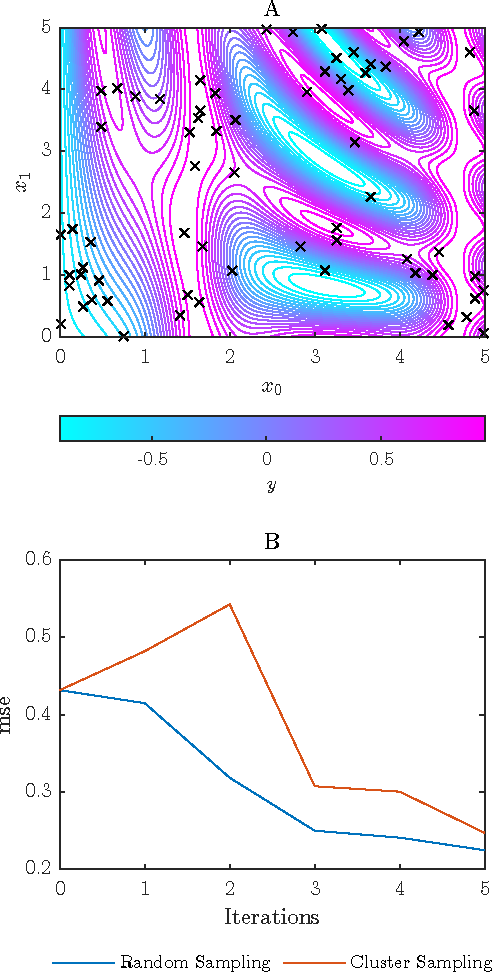
\includegraphics{batchrodPhantom.pdf}
    \caption[Batch Uncertainty Sampling]{The outcome of the investigating the areas of using uncertainty sampling. An initial set of 5 random points was provided, and 5 further iterations were then carried out of sample size 10. A) Demonstrates the final set of points tested by the algorithm and B) shows the change in the mean squared error for the algorithm after each iteration.}
  \end{center}
\end{figure}

\begin{figure}[H]
  \begin{center}
    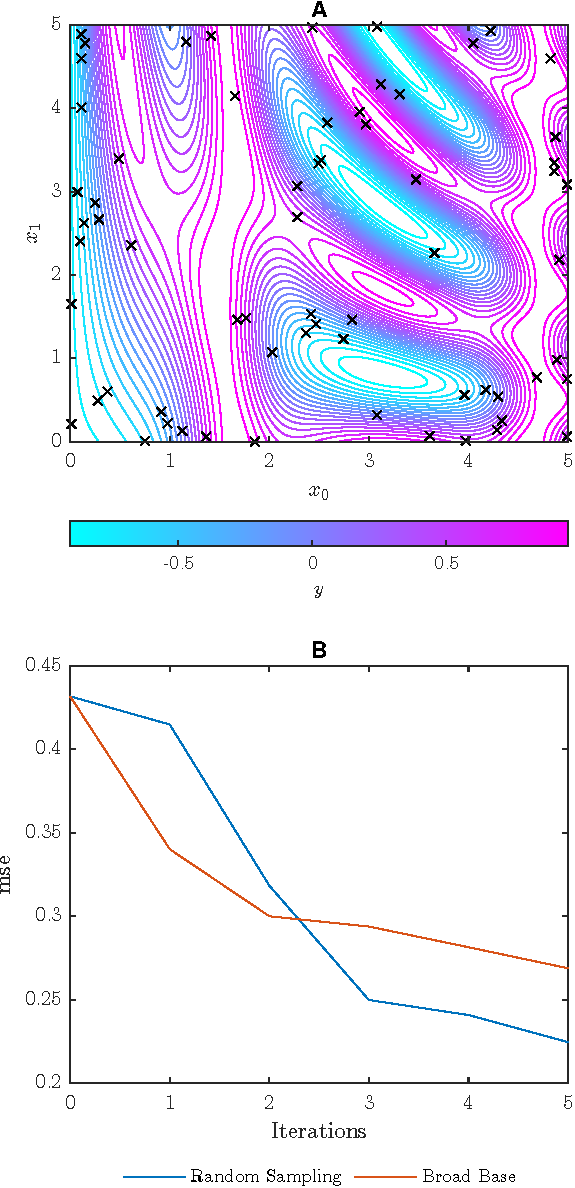
\includegraphics{batchbroadPhantom.pdf}
    \caption[Batch Broad-Base Sampling]{The outcome of the investigating the areas of using broad-base sampling. An initial set of 5 random points was provided, and 5 further iterations were then carried out of sample size 10. A) Demonstrates the final set of points tested by the algorithm and B) shows the change in the mean squared error for the algorithm after each iteration.}
  \end{center}
\end{figure}

\begin{figure}[H]
  \begin{center}
    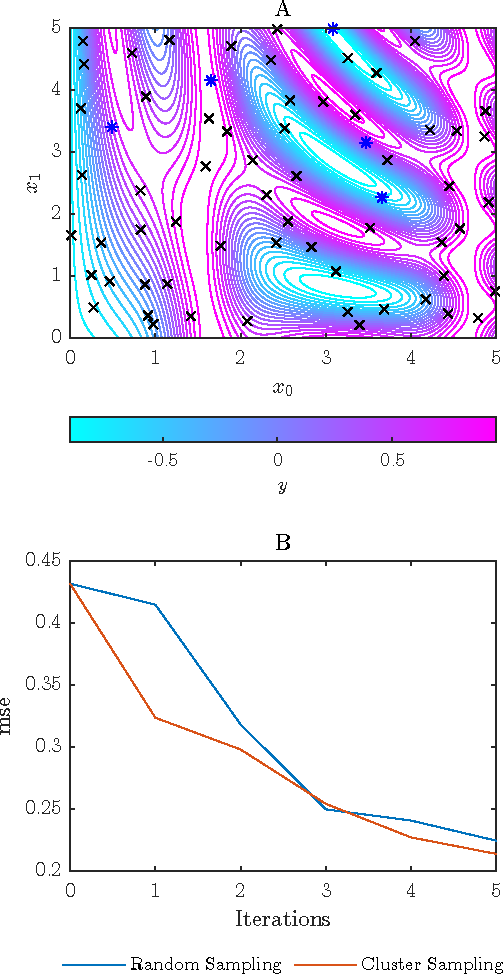
\includegraphics{broadClusterPhantom.pdf}
    \caption[Batch Cluster Sampling]{The outcome of the investigating the areas of using cluster sampling. An initial set of 5 random points was provided, and 5 further iterations were then carried out of sample size 10. A) Demonstrates the final set of points tested by the algorithm and B) shows the change in the mean squared error for the algorithm after each iteration.}
  \end{center}
\end{figure}


It stands to reason that the area which has the highest uncertainty will see this for the data points nearest neighbours. Thus, this singular data point suffers the potential of being surrounded by $N-1$ other data points. The benefit this provides in fitting the model is thus extremely limited, and only slightly greater than if one data point had been chosen. A simple fix would be to simulate the model after 1 iteration, and select the next point from here. By doing this $N-1$ times, a better solution may be found, although this may prove to be computationally very expensive.



\section{Drug Data for Machine Learning}
There are numerous data categories that can be used to represent a chemical in a suitable form for machine learning. Indeed, the field of chemoinformatics is dedicated to the pursuit of describing chemicals for computational models. Each of these methods have various strengths and weaknesses. Some are directly based upon the chemical structure whereas others are based upon physical properties. These can be combined to produce models with high predictive capabilities.

\subsection{Physical Properties}
A selection of physical properties from chemicals are known, from melting points to solubility. Many of these provide important aspects for consideration and allow human scientists to predict interactions, especially when determining new drugs. These data are often reported in tables within textbooks such as Perry's Chemical Engineering Handbook or provided through software \cite{CHEMBL,Perrys}.

Several of these data can be predicted through theoretical models, although the difficulty increases for larger molecules. For example, models exist for density predictions, but predicting the $\mathrm{LD_{50}}$ of a drug is  far more challenging task. Indeed, even with animal testing, this property is deemed difficult to trully assess.

Within drug discovery, physical and biological properties are usually the sought after labels. An example of this is supplied by \textcite{CHEMBL} with a custom property named pChEMBL, as defined by \ref{eq:pChEMBL} where  "|" is synonymous with "or".

\begin{equation}
  \label{eq:pChEMBL}
  \mathrm{pChEMBL}=-\log_{10}{\left(\mathrm{IC_{50}}|\mathrm{XC_{50}}|\mathrm{EC_{50}}|\mathrm{AC_{50}}|\mathrm{Ki}|\mathrm{LD_{50}}|\mathrm{Potency}\right)}
\end{equation}

\subsection{Fingerprints}
Another methodology is to develop a fingerprint: a unique code based on the chemical structure, either of the atomic arrangement, or by the electron cloud distribution. The latter of these is more fundamental to the activity of molecules but far harder to calculate. Indeed, for accurate representation of the latter, both atomic structure is needed \textit{and} solutions for the Schrödinger equations corresponding to molecule in question.

According to \textcite{Cap20}, the most popular fingerprint in use are Morgan Fingerprints, a form of Extended Chemical Fingerprint (ECFP). ECFPs use a simple algorithm in order to generate a unique identifier, as described by \textcite{Mor2020}:

\begin{enumerate}
  \item \textbf{Initial Assignment}: Each atom has an integer assigned as an identifier.
  \item \textbf{Iterative Updating}: Updating the identifier assigned to atoms based on adjacent atoms and structural duplications.
  \item \textbf{Duplicate Removal}: Duplicate features are removed for hashing.
\end{enumerate}

The iteration process involves each atom and adjacent atoms sharing numbers before in an array. A hash function is applied to this array and becomes the atoms new identifier. Fingerprints of this class are labelled according to the number of iterations, $n$, with the final name given as ECFP\_$\langle{}2n\rangle{}$. Morgan fingerprints, the most common form, are thus also called ECFP\_4 \cite{Cap20, Mor2020}. Thus, these come under the remit of fingerprints based upon two-dimensional chemical structure, rather than three-dimensional or even electron distribution. Morgan fingerprints are readily available for millions of compounds from the publicly accessible ChEMBL database \cite{CHEMBL}.

% Alternative common fingerprints include SMILES, InChI, and the MDL molfile.